\documentclass[]{article}
\usepackage[utf8]{inputenc}
\usepackage{polski}
\usepackage{graphicx}
\graphicspath{ {./images/} }
\usepackage[margin=0.5in]{geometry}
\usepackage{gensymb}
\usepackage{textcomp}
\usepackage{siunitx}
\usepackage{float}
\documentclass{article}
\usepackage{graphicx}
\usepackage{wrapfig}
\usepackage{lipsum}
\usepackage{graphicx}
\usepackage{subcaption}
\begin{document}

\begin{figure}[tp!]
	\center{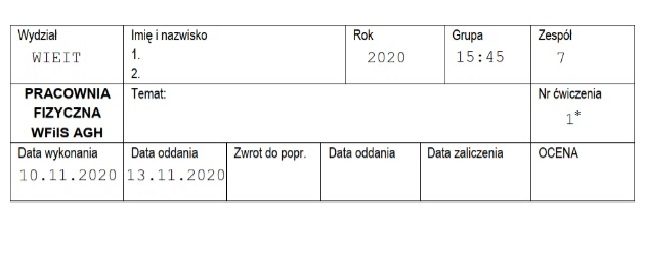
\includegraphics{Name_Card}}
\end{figure}

\begin{center}
	\section*{Wahadło fizyczne}
	\emph{Dzmitry Mikialevich}
\end{center}
\begin{center}
	\emph{Wojciech Sikora}
\end{center}
\tableofcontents
\newpage

\section{Wstęp}

\subsection{Cel ćwiczenia}
Opis ruchu drgającego, a w szczególności drgań wahadła fizycznego. Wyznaczenie momentów
bezwładności brył sztywnych.

    


\section{Układ Pomiarowy}
W skład układu pomiarowego weszły następujące elementy:
\newline

1.Pudełko tekturowe po herbacie uszczelnione plastikowym woreczkiem szczelnie wypełnionym solą

2.Patyczek do szaszłyków

3. Dwa stosy książek

4. Stoper w smartfonie

\begin{figure}[h!]
  \centering
  \begin{subfigure}[b]{0.4\linewidth}
    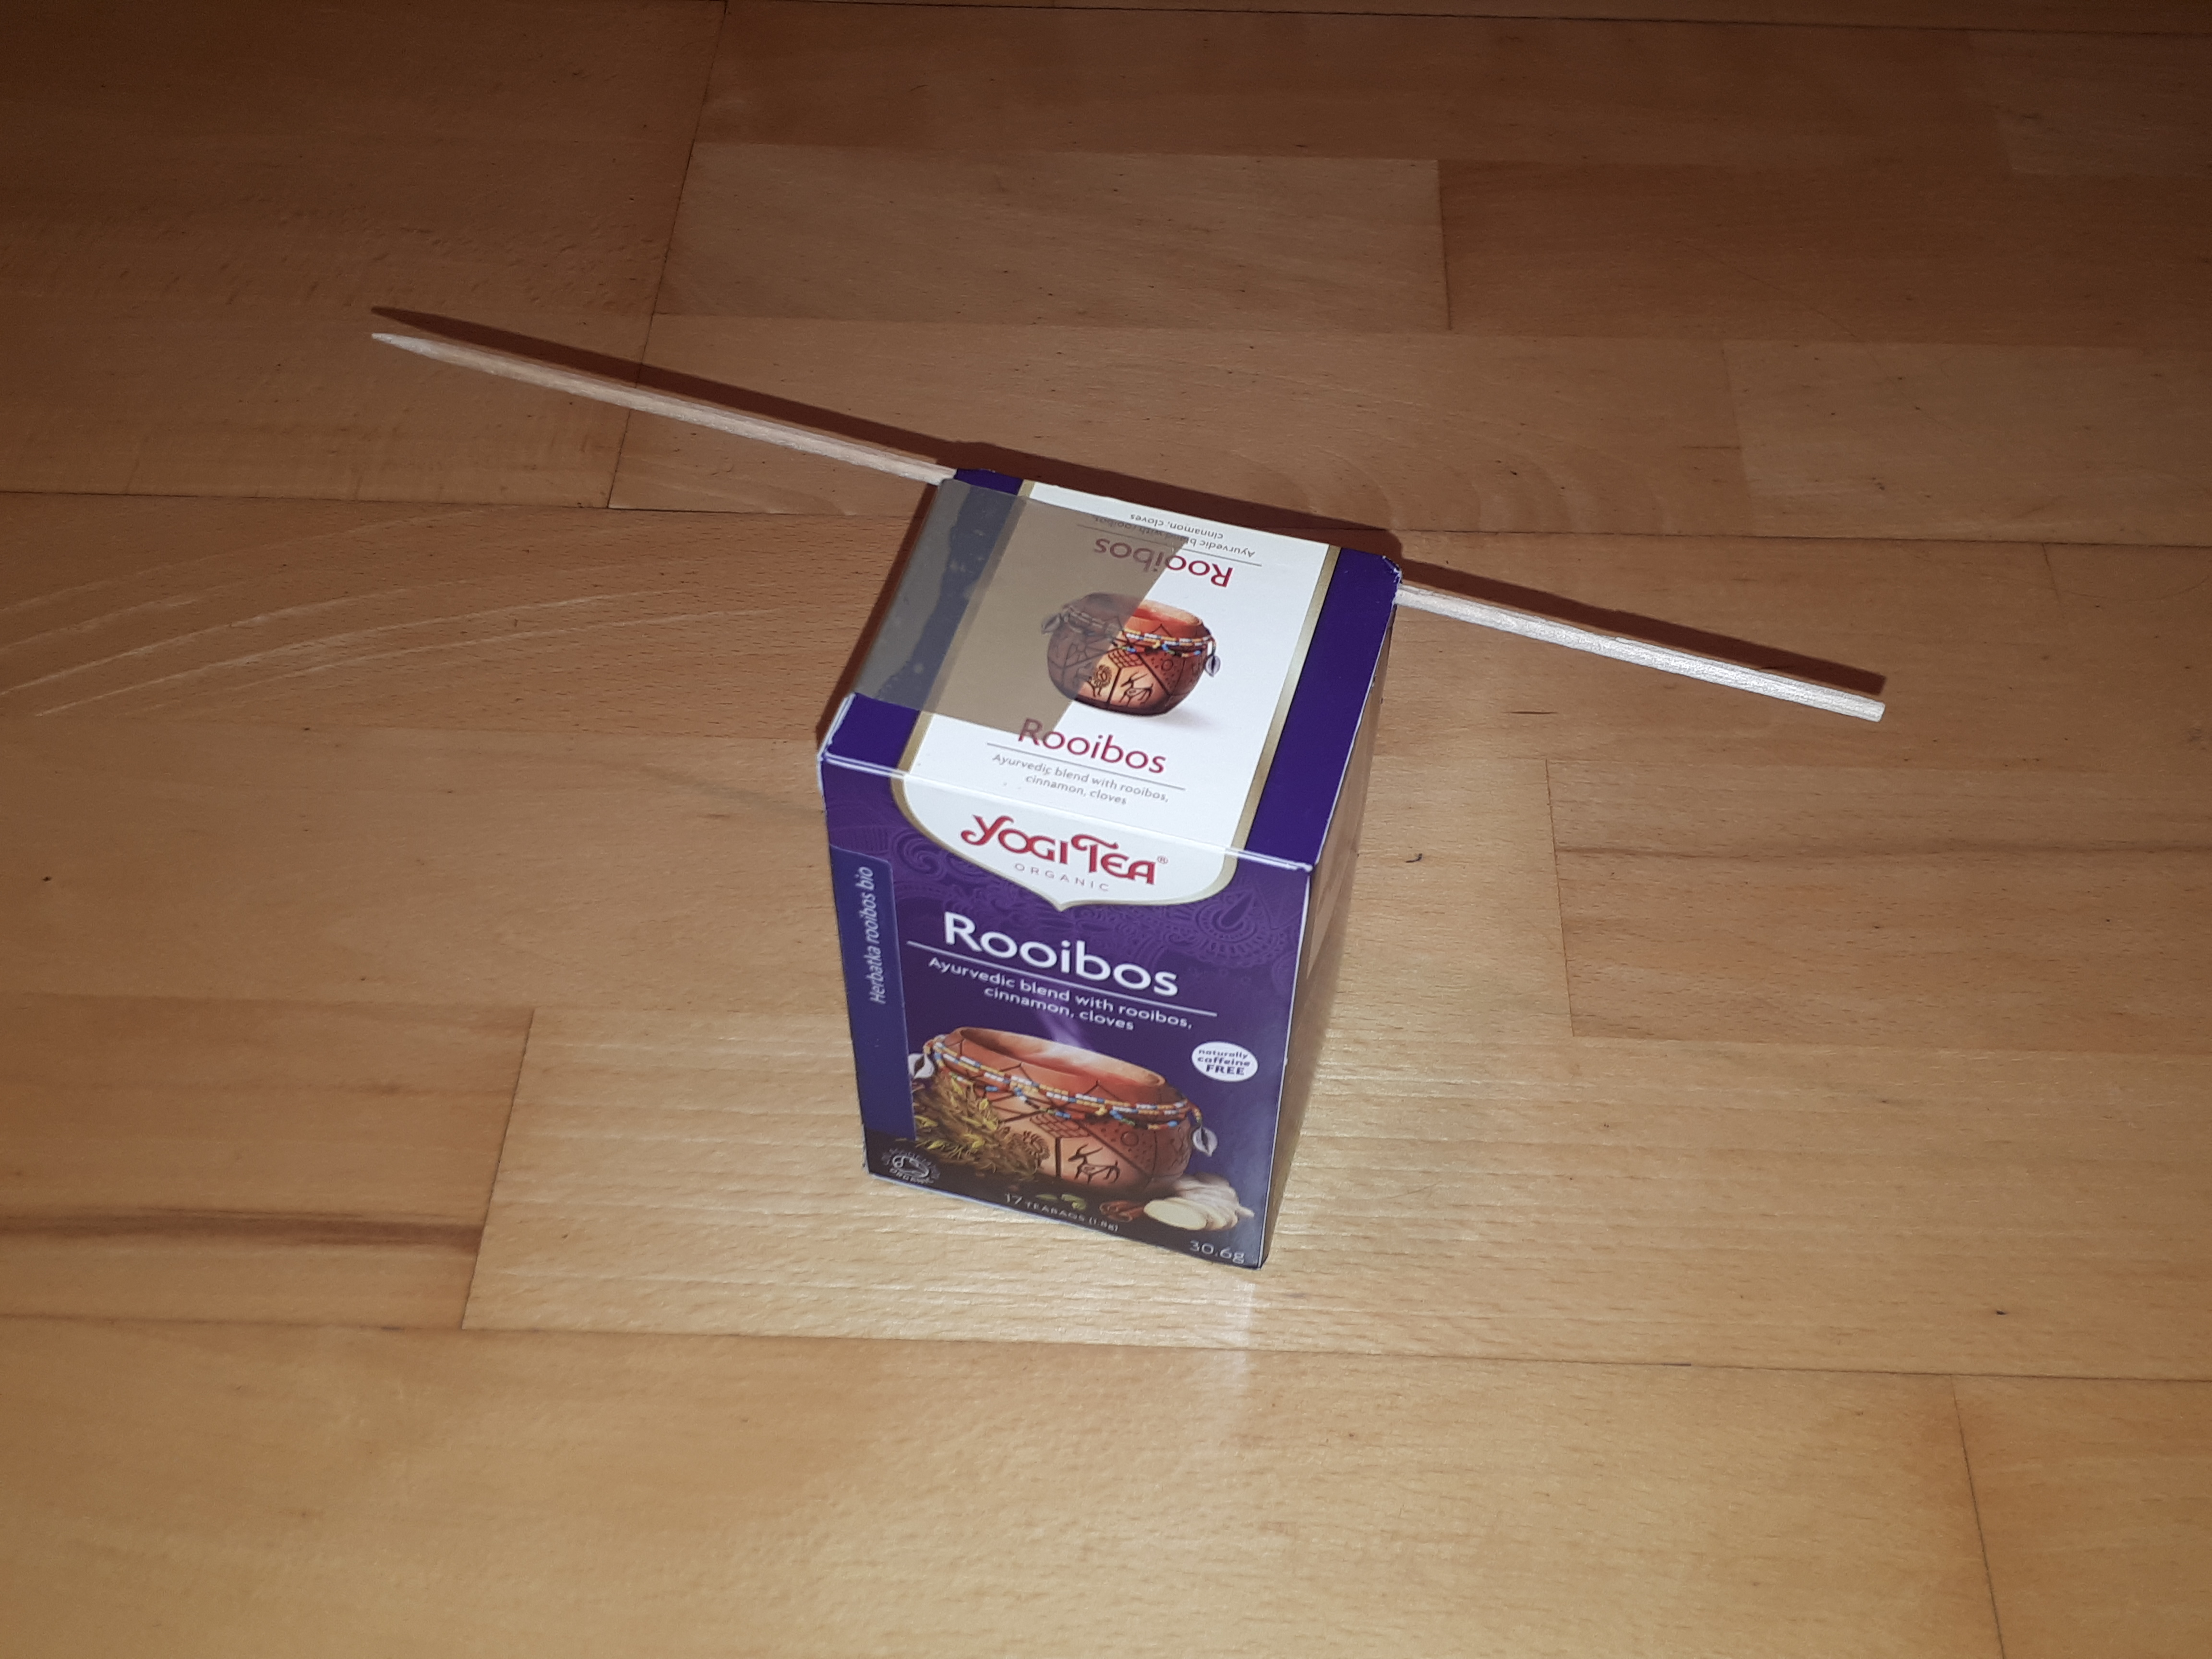
\includegraphics[width=\linewidth]{1}
    \caption{Pudełko tekturowe wraz z patyczkiem}
  \end{subfigure}
  \begin{subfigure}[b]{0.4\linewidth}
    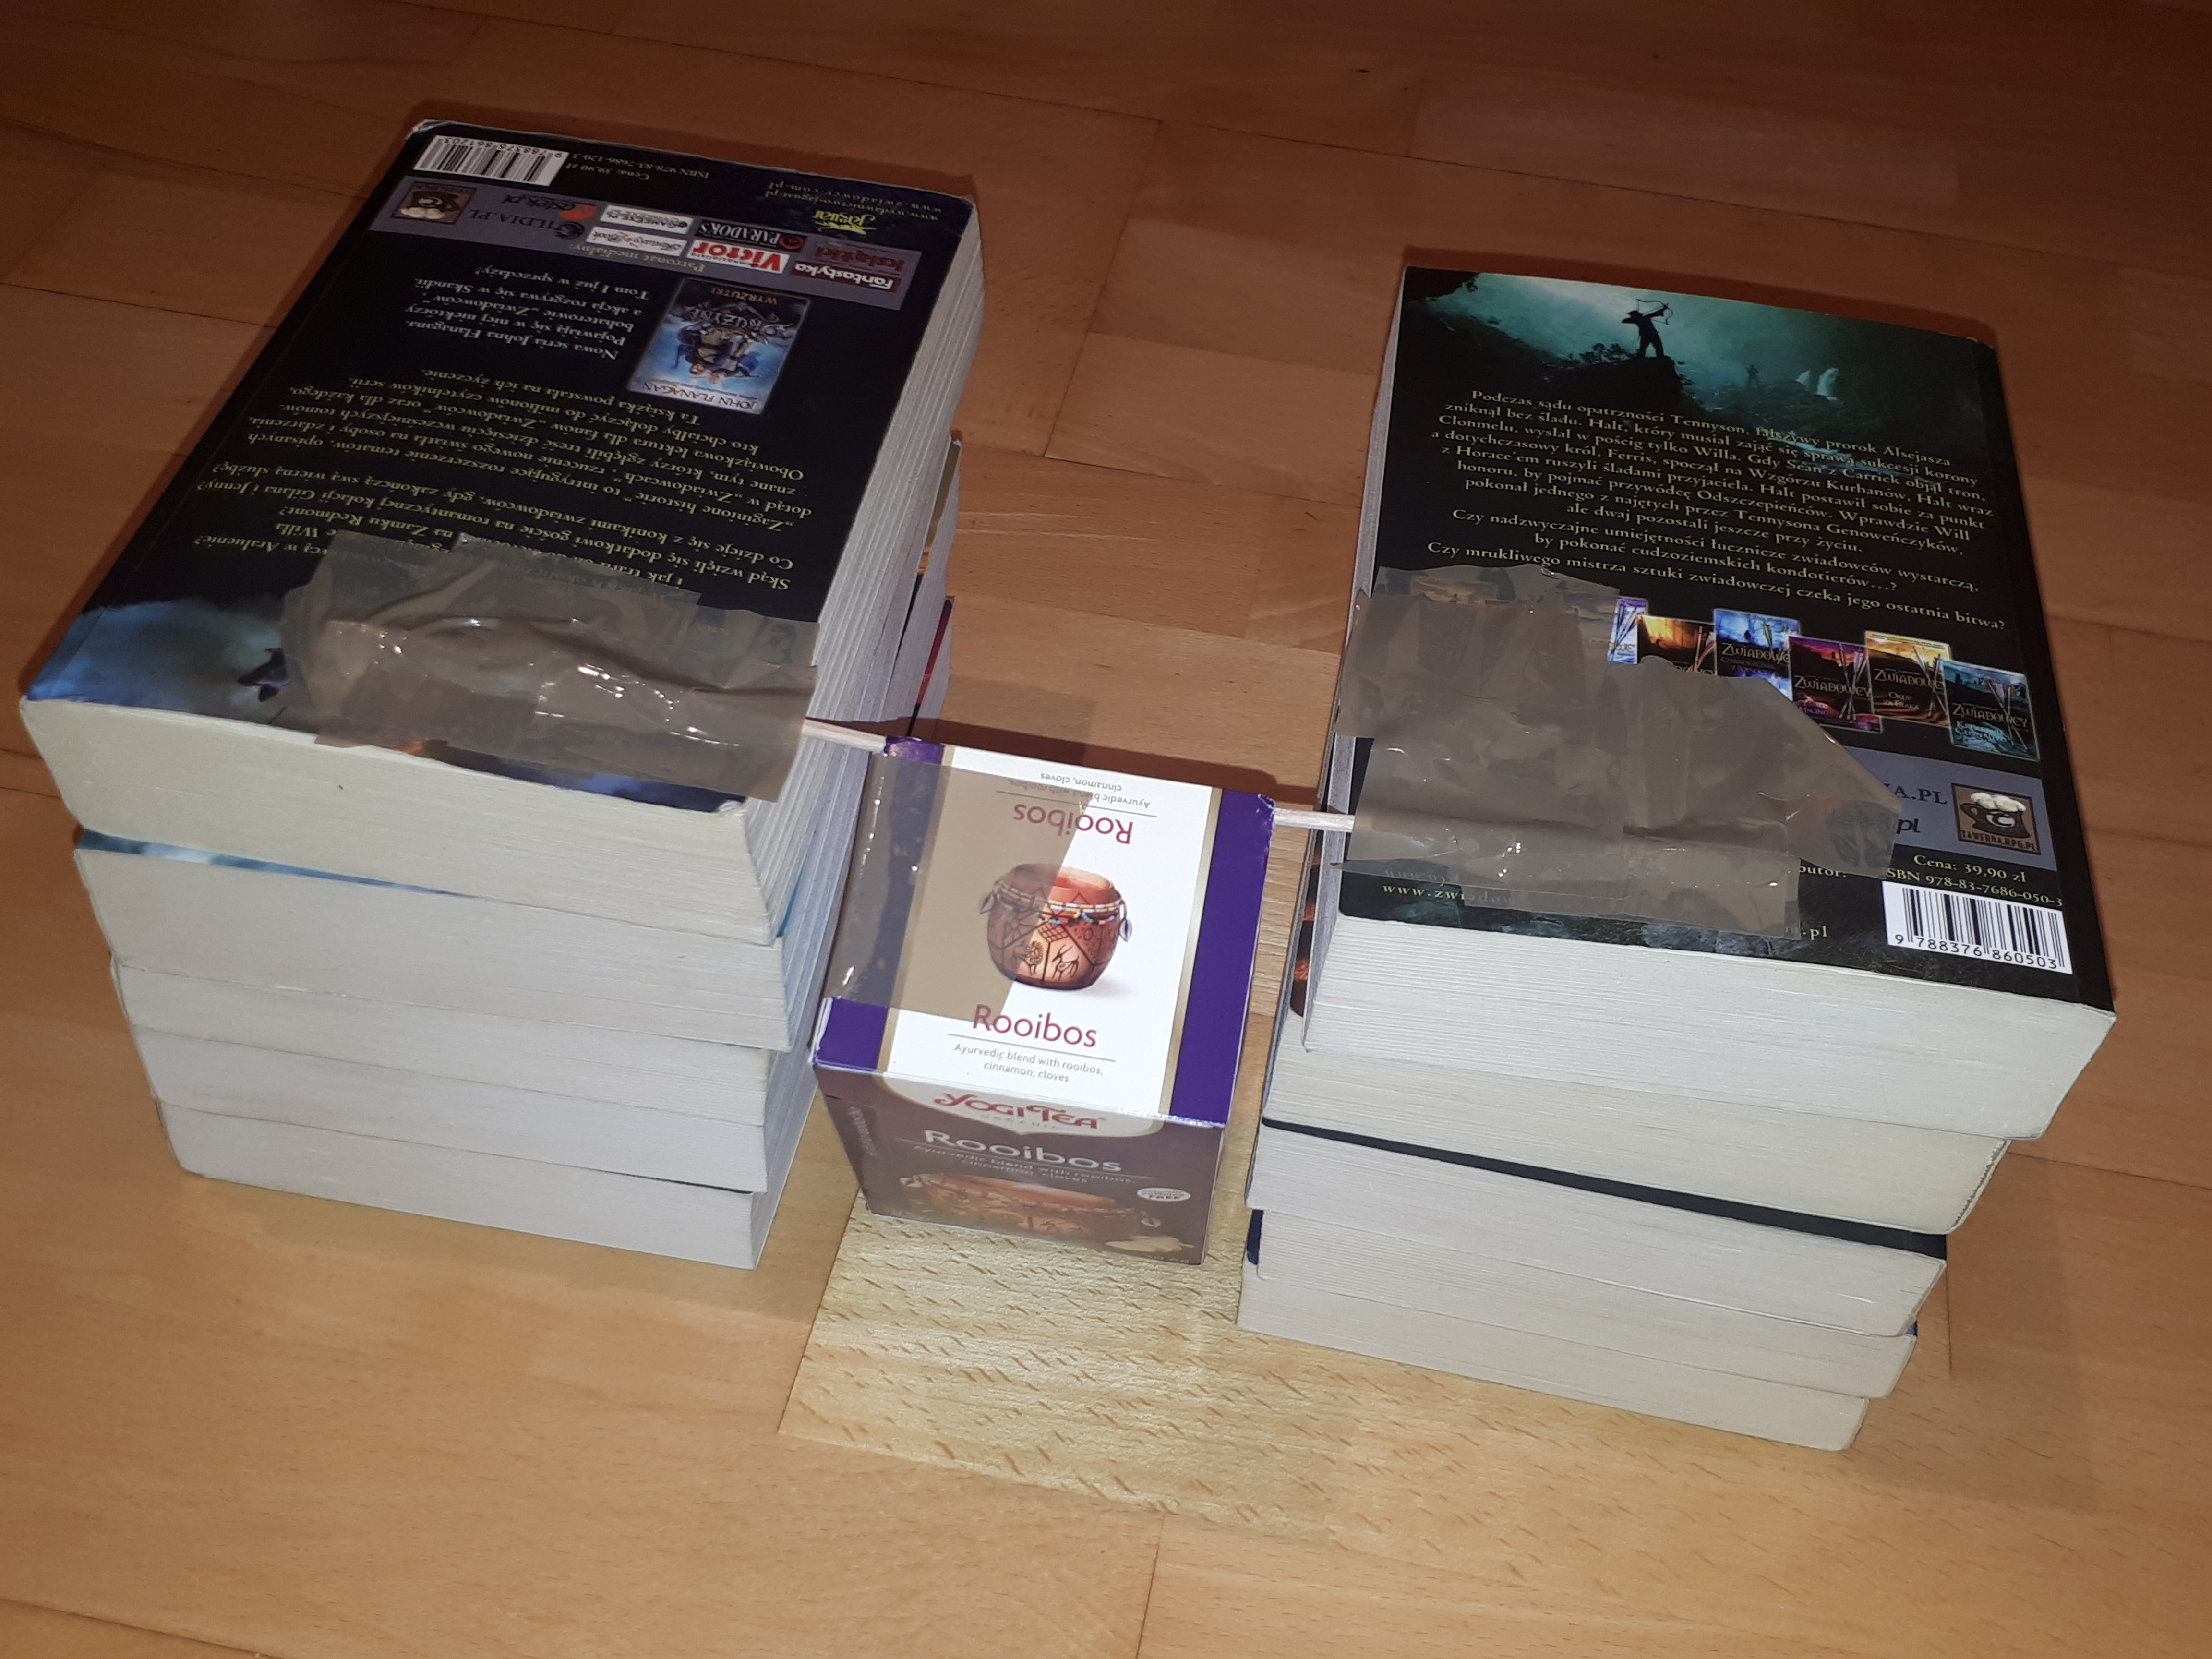
\includegraphics[width=\linewidth]{2}
    \caption{Patyczek z pudełkiem podparty na stosach książek}
  \end{subfigure}
  \begin{subfigure}[b]{0.4\linewidth}
    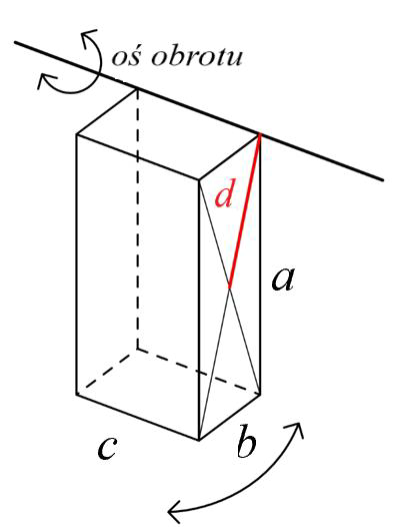
\includegraphics[width=\linewidth]{4}
    \caption{Schemat układu}
  \end{subfigure}
  \begin{subfigure}[b]{0.4\linewidth}
    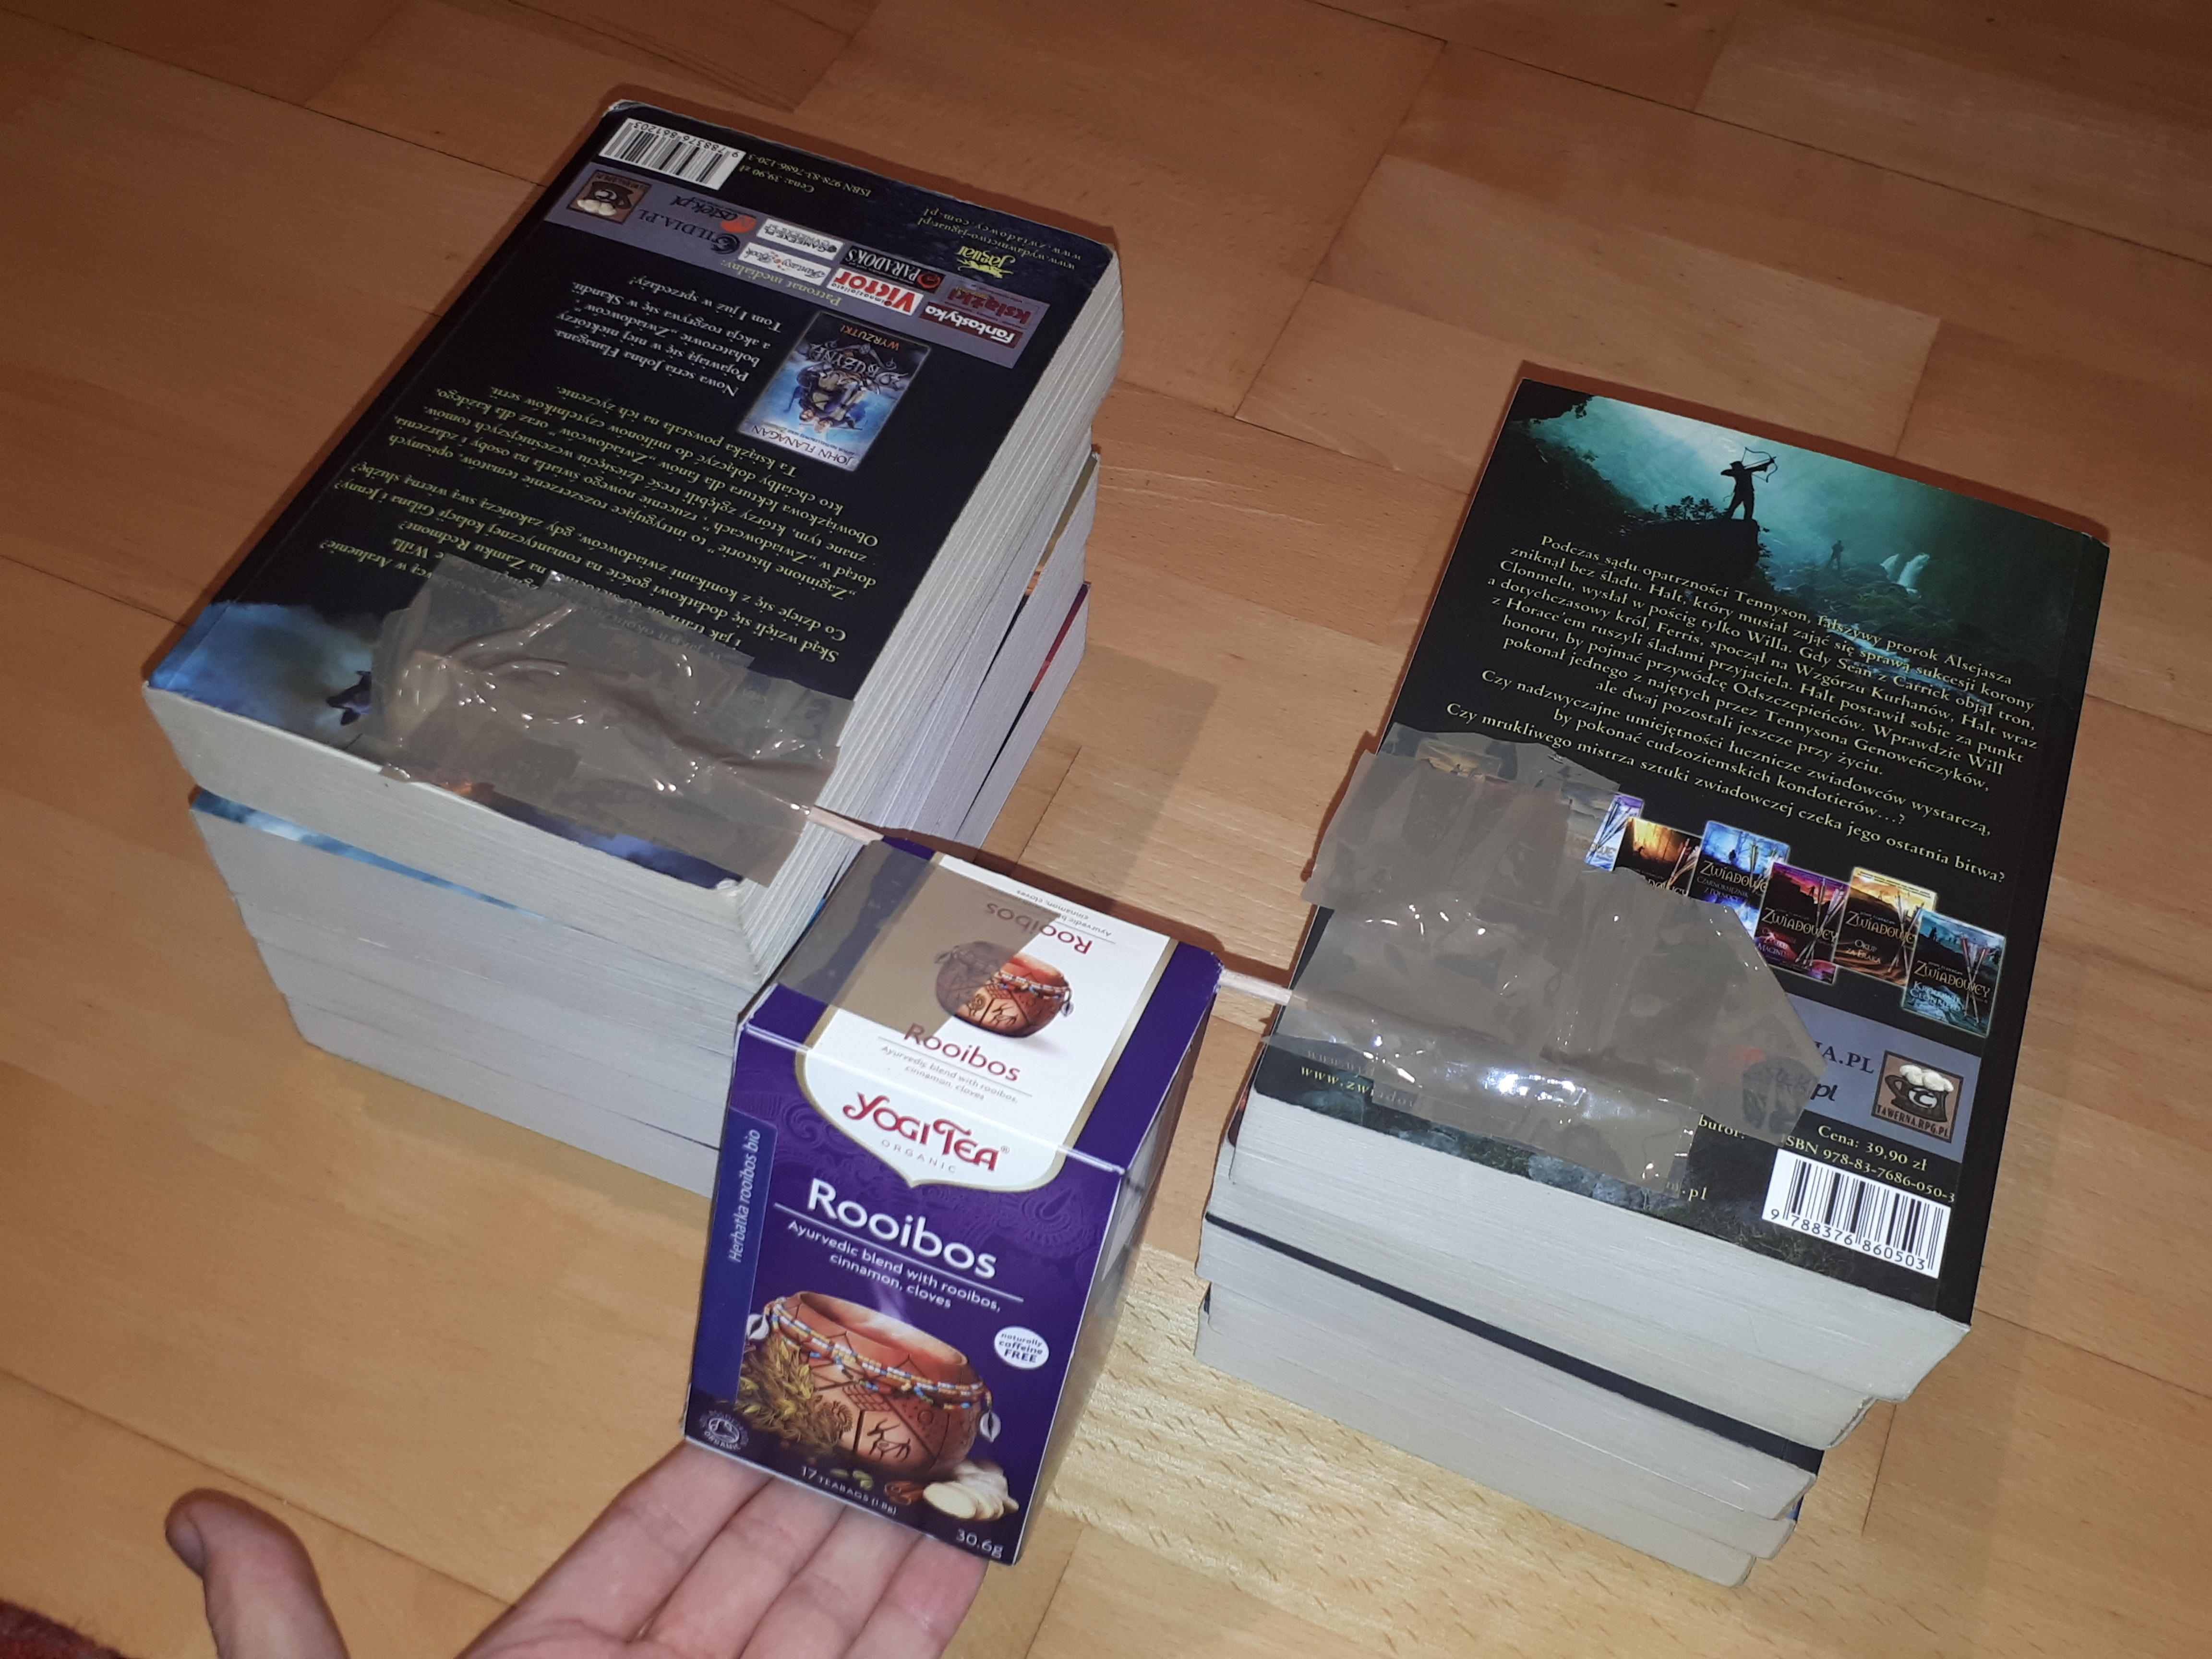
\includegraphics[width=\linewidth]{3}
    \caption{Wprawianie bryły w ruch drgający}
  \end{subfigure}
  
\end{figure}


% \begin{figure}[H]
% \begin{wrapfigure}{l}{0.3\textwidth}\centering
% 	\center{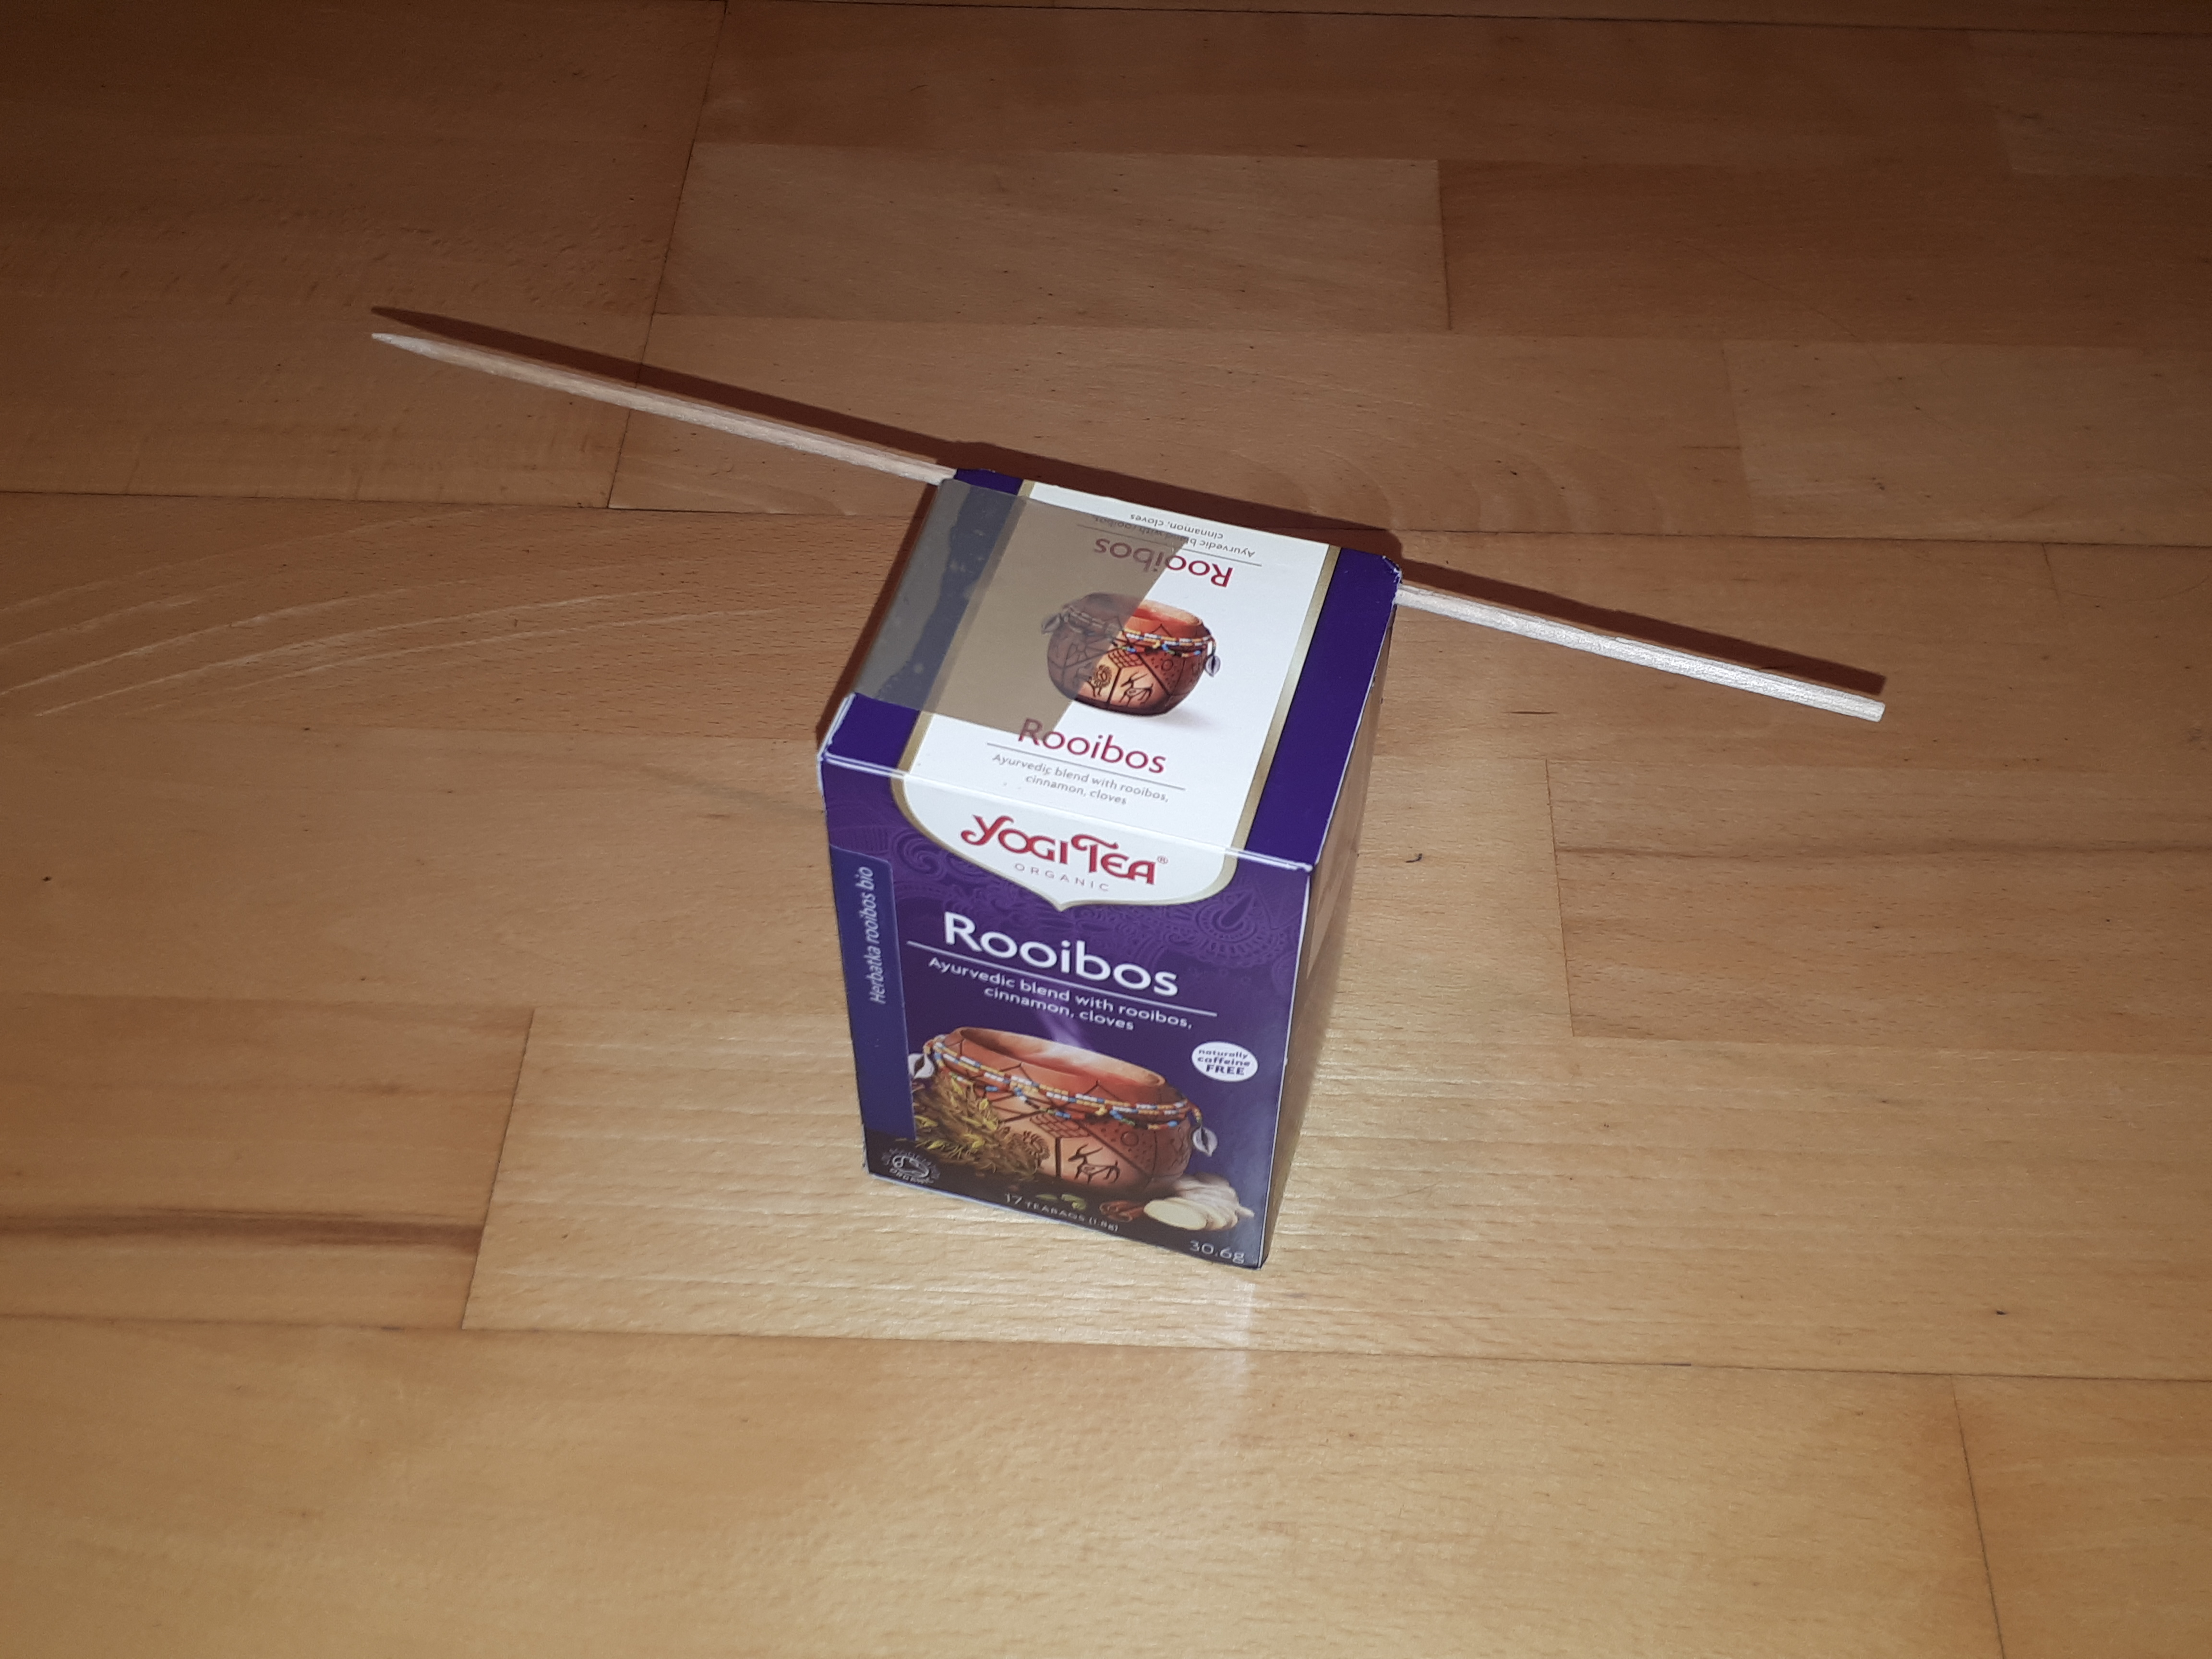
\includegraphics[scale = 0.05]{1}

	
	
% 	\textbf{\caption{Badany układ rury Quinckego}}
% 	\end{wrapfigure}
	
% \end{figure}


% \begin{figure}[H]
% \begin{wrapfigure}{t}{0.3\textwidth}\centering
% 	\center{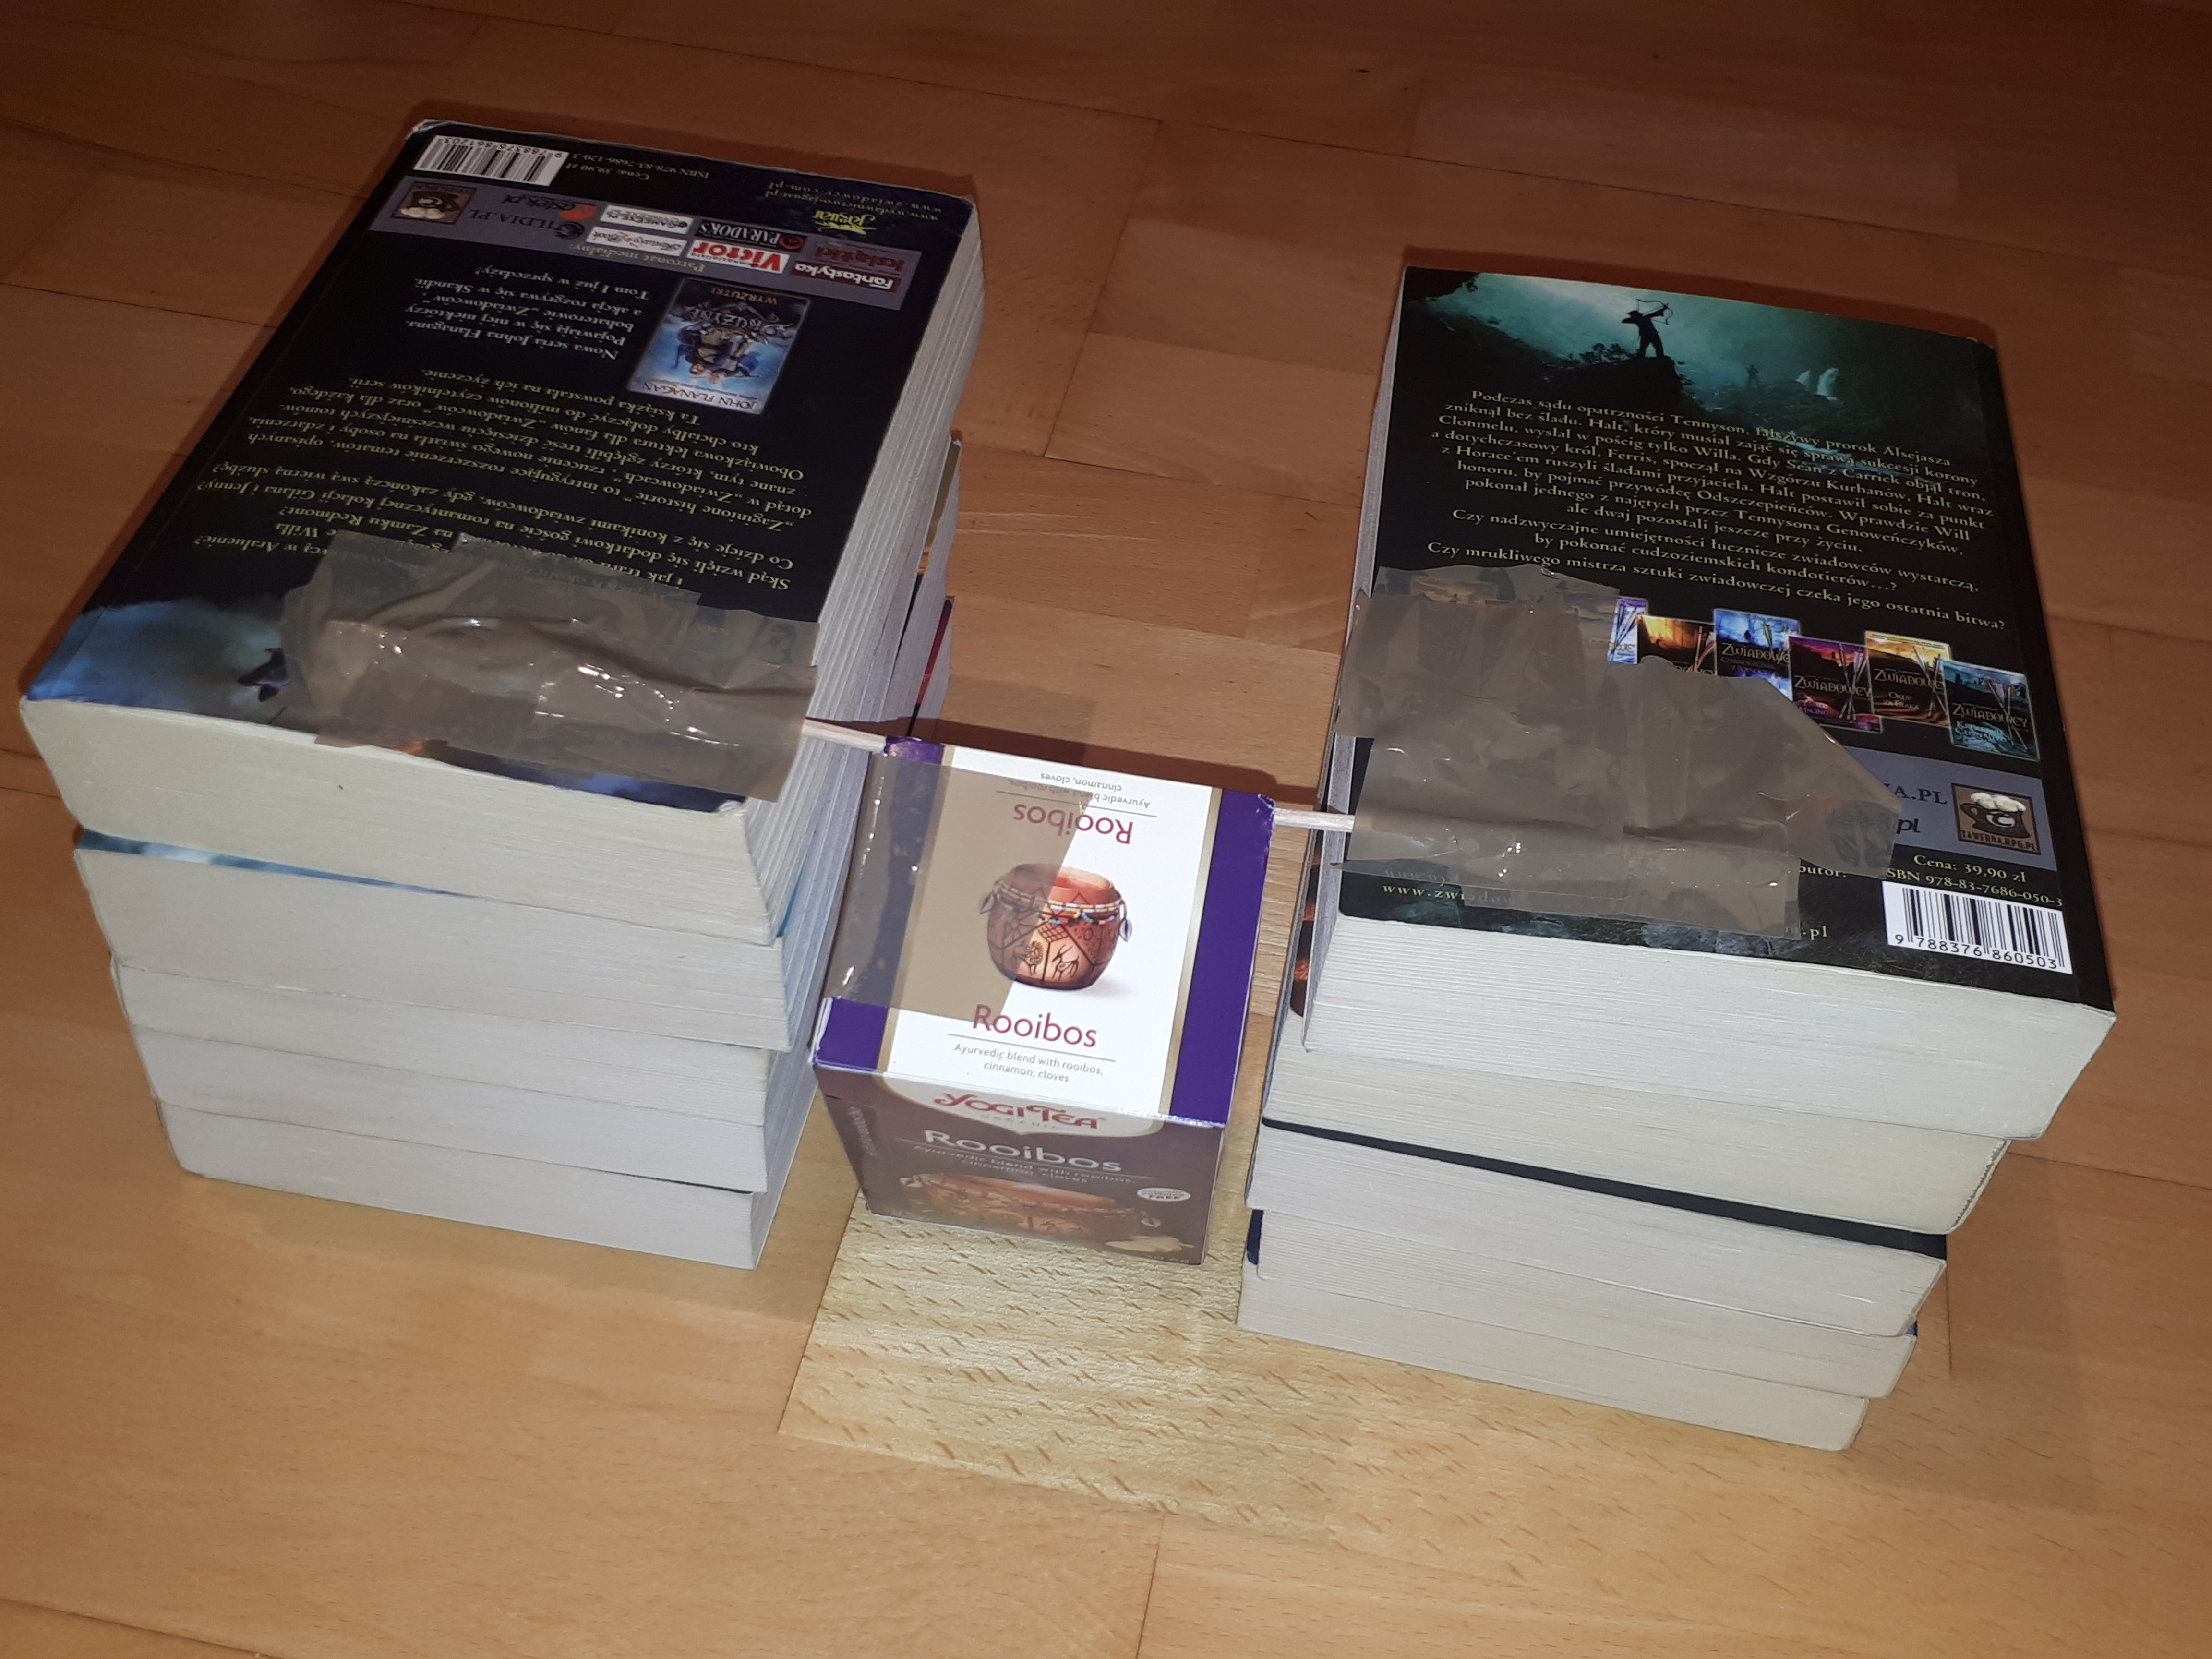
\includegraphics[scale = 0.05]{2}{contour}}
% 	\textbf{\caption{Badany układ rury Quinckego}}
% 	\end{wrapfigure}
	
% \end{figure}

% \begin{figure}[H]
% 	\center{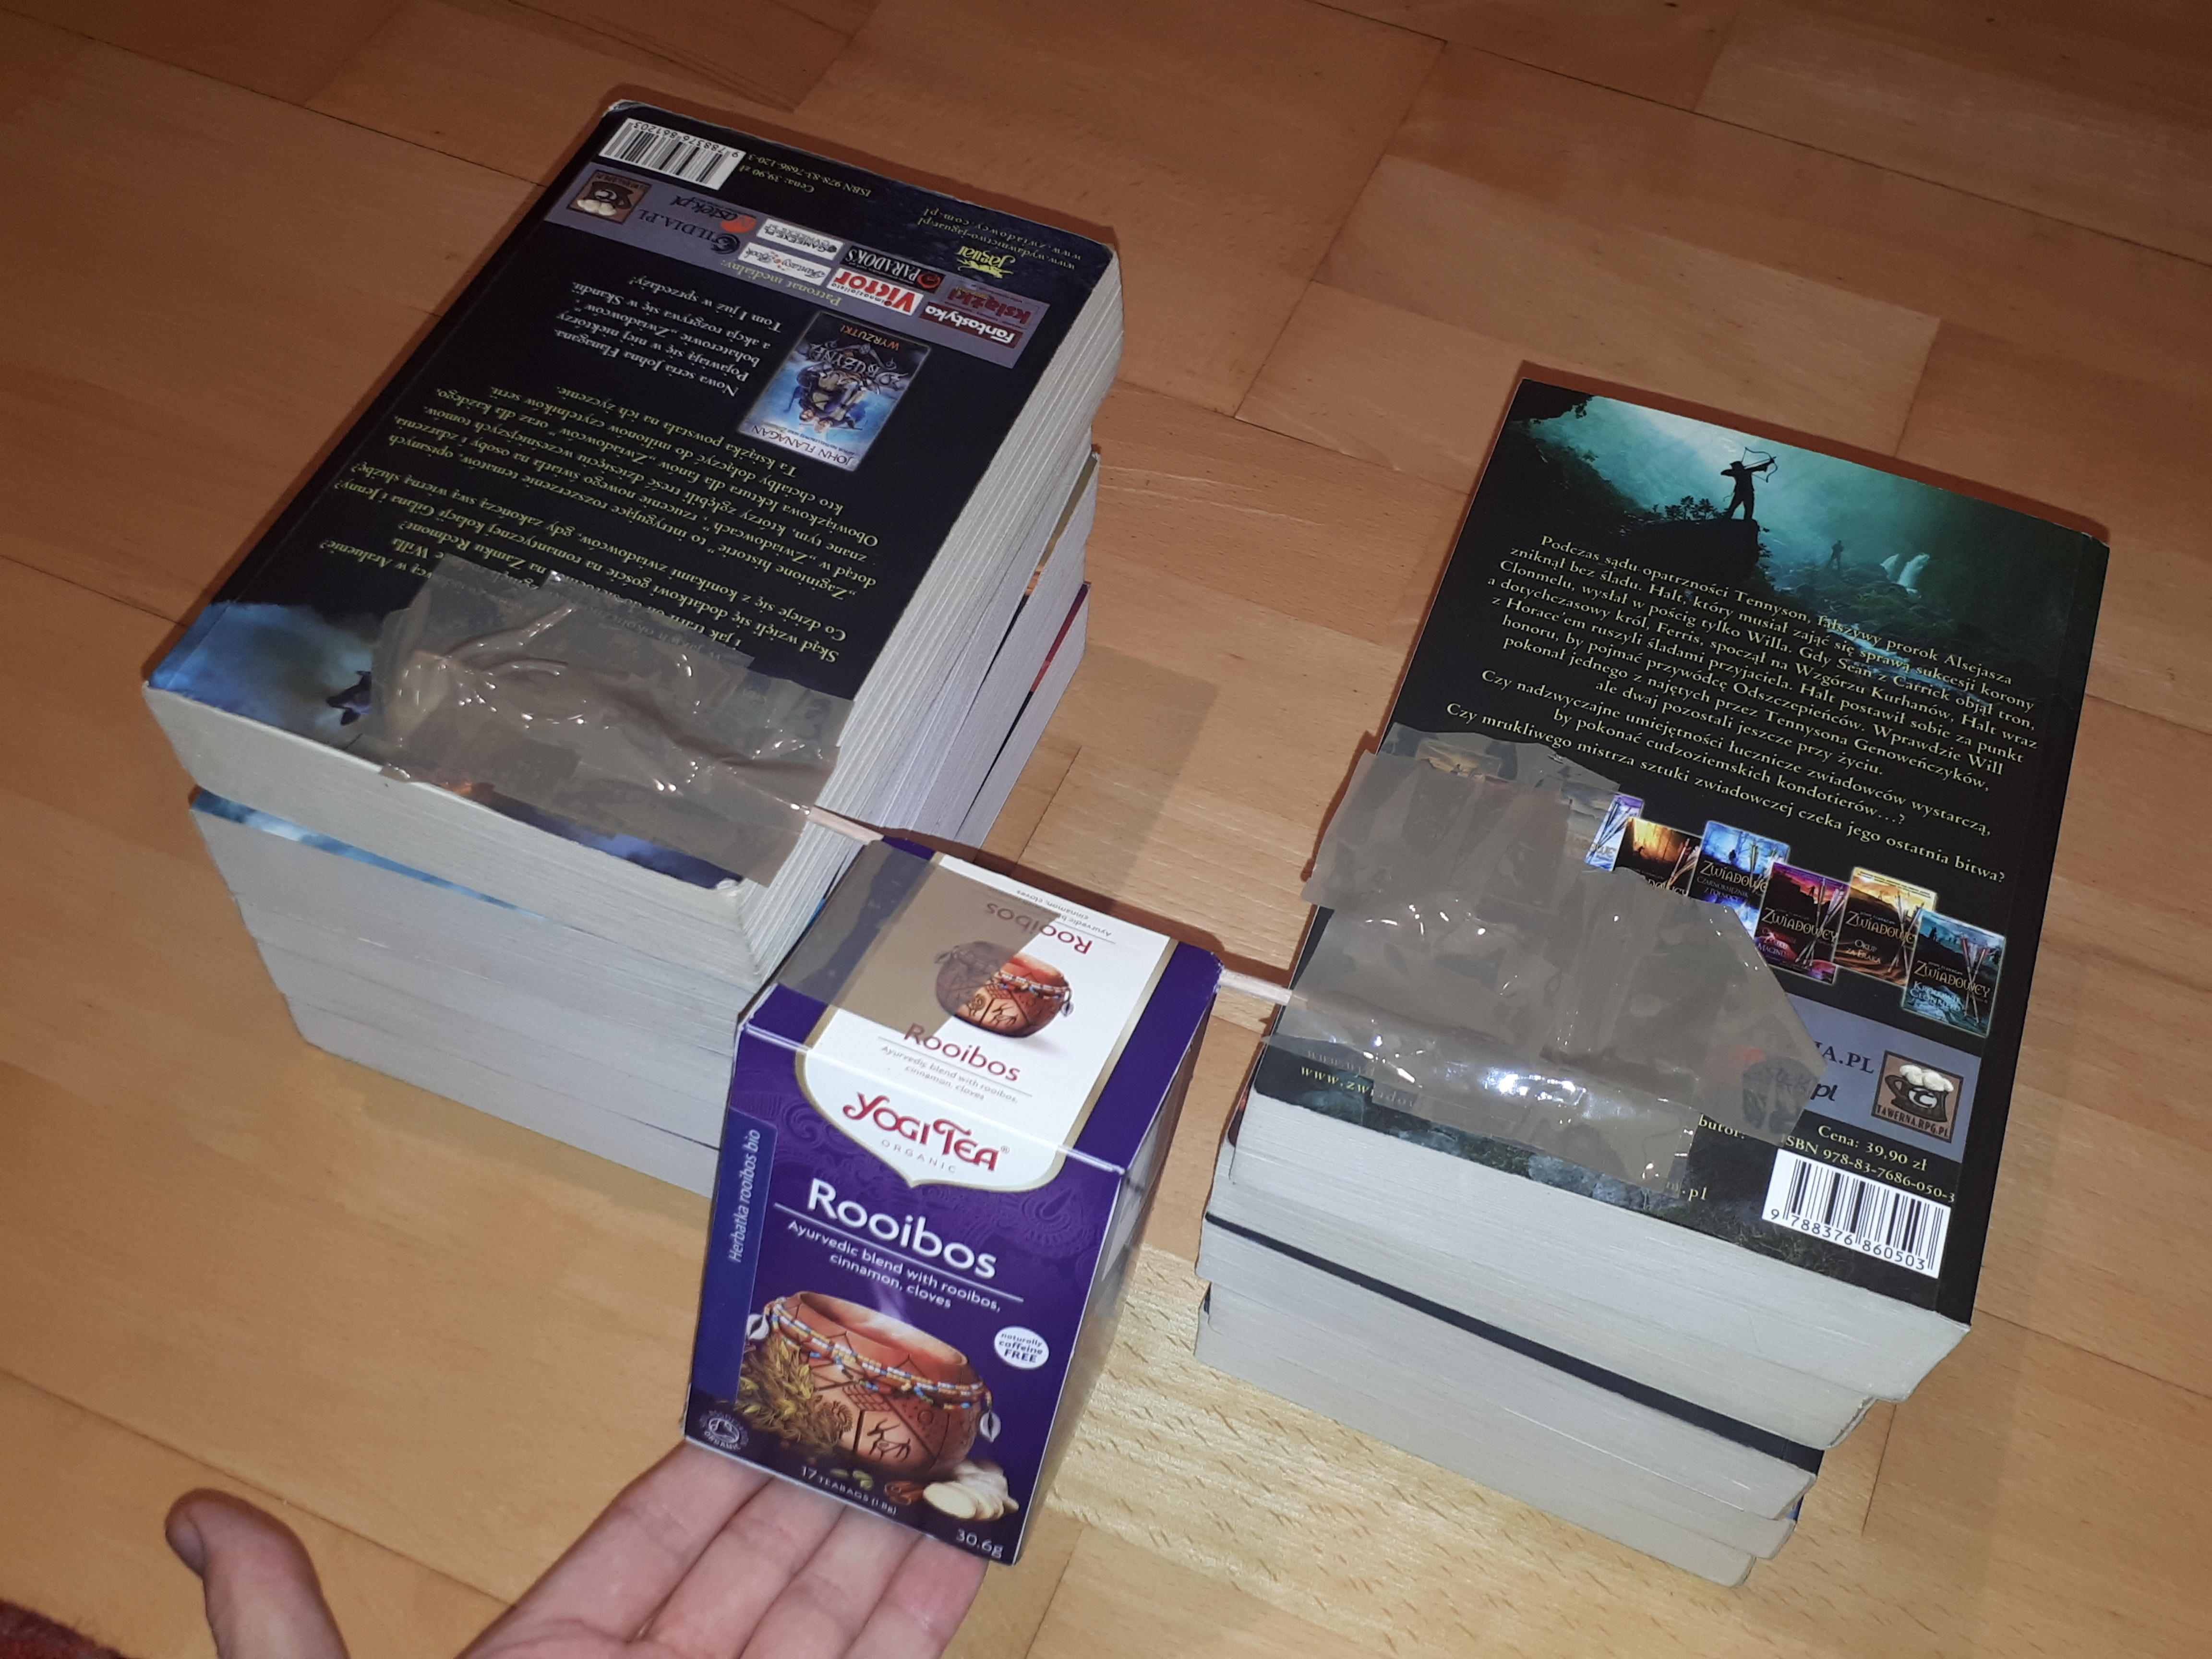
\includegraphics[scale = 0.05]{3}}
% 	\textbf{\caption{Badany układ rury Quinckego}}
	
% \end{figure}




\section{Przebiegi doświadczenia}
W ramach doświadczenia na początku wypełniliśmy solą uszczelnione plastikowym woreczkiem pudełko po herbacie. Aby pudełko miało postać stabilnego prosotpadłościanu skleiliśmy taśmą klejącą bok pudełka, który służył jako jego otwarcie. Przy pomocy wagi kuchennej zważyliśmy taką bryłę. Następnie zmierzyliśmy długości boków a, b oraz wyznaczyliśmy odległość d konieczną do skorzystania z twierdzenia Steinera.

Następnie umieściliśmy pudełko prostopadłościanu na podpórkach, podpierając oś końcami na równych stosach książek, tak aby miała możliwość swobodnego obrotu.
Wprawialiśmy bryłę w drganie dwudziestokrotnie i mierzyliśmy czas kilkunastu okresów.

\section{Wyniki Pomiarów}
  
   
   	\begin{table}[h]
		\centering
		\begin{tabular}{|l|l|l|}
			\hline
 & wartość & niepewność\\ \hline
Masa m [kg] & 0,590 & 0,001 \\ \hline
a [m] & 0,118 & 0,001 \\ \hline
b [m] & 0,069 & 0,001   \\ \hline
d [m] & 0,635 & 0,001  \\ \hline


		\end{tabular}
		\textbf{\caption{Wyniki pomiarów masy i długości}
		}
	\end{table} 

	\begin{table}[h]
		\centering
		\begin{tabular}{|l|l|l|l|}
			\hline
L.p & Ilość okresów & Czas [s] & Okres T [s]\\ \hline
1 & 21 & 12,93 &  0,6157 \\ \hline
2& 15 & 9,18 &  0,6120 \\ \hline
3 & 26 & 15,59 &  0,5996 \\ \hline
4 & 20 & 12,42 &  0,6210 \\ \hline
5 & 20 & 11,83 &  0,5915 \\ \hline
6 & 22 & 13,08  & 0,5945 \\ \hline
7 & 27 & 16,26 &  0,6022 \\ \hline
8 & 23 & 13,87 &  0,6030 \\ \hline
9 &  24 & 14,13 & 0,5888 \\ \hline
10 & 21 & 12,51 & 0,5957 \\ \hline
11 & 25 & 14,73 & 0,5892 \\ \hline
12 & 25 & 14,97 &  0,5988 \\ \hline
13 & 22 & 13,15 &  0,5977 \\ \hline
14 & 19 & 11,21 &  0,5900 \\ \hline
15 & 27  & 16,17 & 0,5989 \\ \hline
16 & 21 & 12,73 &  0,6062 \\ \hline
17 & 23 & 13,82 &  0,6009 \\ \hline
18 & 24 & 14,34 &  0,5975 \\ \hline
19 & 22 & 13,19 &  0,5995 \\ \hline
20 & 25 & 14,89 &  0,5956 \\ \hline
\multicolumn{3}{|c|} {Średni Okres [s]} & 0,6000  \\ \hline
\multicolumn{3}{|c|} {Niepewność u(T) [s]} & 0,0019  \\ \hline
% TODO D
		\end{tabular}
		\textbf{\caption{Wyniki pomiarów okresu drgań}
		}
	\end{table}
\newline



\section{Opracowanie wyników Pomiarów}
    \subsection{Moment bezwładności \(I_0\)}

Moment bezwładności \(I_0\) względem rzeczywistej osi obrotu korzystając z wzoru na okres drgań:
    \[T = 2\pi \sqrt{\frac{I_0}{mgd}} \Rightarrow I_0 = \frac{mgdT^2}{4\pi^2} = 0,003351487 \approx 0,0034\:[kg*m^2]\]
\[
u_c(I_0) = \sqrt{
    (\frac{\partial l_0}{\partial m} * u(m))^2 + 
    (\frac{\partial l_0}{\partial d} * u(d))^2 + 
    (\frac{\partial l_0}{\partial T} * u(T))^2
}
= 0,005175634 \approx 0,0052 \:[kg*m^2]
\]
    \subsection{Moment bezwładności \(I_s\)}
Moment bezwładności \(I_s\) względem osi przechodzącej przez środek masy i równoległej do osi obrotu w wykonanym doświadczeniu:
    \[I_s = I_0 - md^2 = 0,000972459 \approx 0,0010\:[kg*m^2]\]
    \[
u_c(I_{s}) = \sqrt{
    (\frac{\partial I_{s} }{\partial I_0} u(I_0))^2 + 
    (\frac{\partial I_{s} }{\partial m} u(m))^2 + 
    (\frac{\partial I_{s} }{\partial d} u(d))^2
}
\]
\[
u_c(I_{s}) = \sqrt{
    (u(I_0))^2 + 
    (-d^2 u(m))^2 + 
    (-2mdu(d))^2
}
 = 0,005010055 \approx 0,0051 [kg * m^2]
\]
    \subsection{Moment bezwładności \(I_{s(geom)}\)}
Moment bezwładności \(I_{s(geom)}\) względem osi przechodzącej przez środek masy, tym razem na podstawie znanej masy i wymiarów geometrycznych:
    \[I_{s(geom)} = \frac{1}{12}m(a^2 + b^2) = 0,0009187\:[kg*m^2] \approx 0,000919\:[kg*m^2] \]
\[
u_c(I_{s(geom)}) = \sqrt{
    (\frac{\partial I_{s(geom)} }{\partial m} u(m))^2 + 
    (\frac{\partial I_{s(geom)} }{\partial a} u(a))^2 + 
    (\frac{\partial I_{s(geom)} }{\partial b} u(b))^2
}
\]
\[
u_c(I_{s(geom)}) = \sqrt{
    (\frac{1}{12} (a^2 + b^2) u(m))^2 + 
    (\frac{1}{6} m a u(a))^2 + 
     (\frac{1}{6} m b u(b))^2 
} = 0,0000135313738382837 \approx 0,000014  \:[kg*m^2]

\]
    \subsection{Niepewności}
Niepewności typu B:
\[u(m) = 0,001\: kg\]
\[u(a) = u(b) = u(d) = 0,001\:m\]
\[u(t) = 0,01\:s\]
Niepewności typu A:
\[u(T) =\sqrt{\frac{\sum{(T_i - \overline T)^2}}{n(n-1)}} = 0,00181738\:s \approx 0,0019\:s\]

    \subsection{Porównanie}
Sprawdzenie czy uzyskane wyniki dla \(I_s\) i \(I_{s(geom)}\) mieszczą się w granicach niepewności rozszerzonej, skorzystamy z zależności:

\[
U(I_{s(geom)} - I_{s}) = k \sqrt{(u(I_{s(geom)})^2 + u( I_{s})^2}
= 0,01036525\:[kg*m^2] \approx 0,011\:[kg*m^2]
\]
\[
|I_{s(geom)} - I_{s}| = 0,000081 << 0,01036525 \approx 0,011\:[kg*m^2]
\]
Czyli wyniki pomiaru można uważać za zgodnę ze sobą.









\section{Wnioski}
\begin{itemize}
        \item Korzystając z wzoru na okres drgań obliczyliśmy wartość momentu bezwładności \(I_{0}=0,0034\:[kg*m^2]\).\newline Niepewność \(u_{c(I_{0})}=0,0052\:[kg*m^2]\)
        
		\item Korzystając z twierdzenia Steinera obliczyliśmy moment bezwładności \(I_{s}\) względem osi przechodzącej przez środek masy i równoległej do osi obrotu w wykonywanym doświadczeniu.\newline Wartość \(I_{s}= 0,0010\: [kg*m^2]\). Niepewność \(u_c(I_{s})=0,0051|\:[kg*m^2]\)
		\item  Wartość \(I_{s(geom)}= 0,000919\: [kg*m^2]\). Niepewność \(u_c(I_{s(geom)})=0,000014|\:[kg*m^2]\)
		\item  Można zauważyć, że wartość momentu bezwładności \(I_{s}\) nieznacznie różni się od wartości momentu bezwładności \(I_{s(geom)}\). Świadczy to o prezycji dokonanych pomiarów okresu drgań wahadła fizycznego.
		\item Dokładniejszą metodą wyznaczenia momentu bezwładności jest metoda geometryczna.
	\end{itemize}
\end{document}
